% Created by Matthew Riehl
% License: MIT
%


\documentclass[]{article}
\usepackage{fullpage}
\usepackage{tikz}
\usepackage{amsmath}
\usepackage{pgfplots}
\pgfplotsset{compat=newest}
\title{}
\author{Dr. Matthew Riehl}
\date {17 March 2021}



\begin{document}
	
	\section*{Projectile Motion}
	Motion of object with $x$-component and $y$-component which are independent of each other.  Can  be described with parametric equations ($x=f(t)\ \text{and }y=f(t)$).  Initial velocity is: $$\vec{v}_0=v_{0x}\hat\i+v_{0y}\hat\j$$ and $x$- and $y$-components are $$v_{x0}=v_0\cos{\theta _0}\text{ and }v_{y0}=v_0\sin{\theta _0}$$ where $\theta _0$ is the angle between $v_0$ and the positive $x$ direction.
	
	
	\begin{center}
		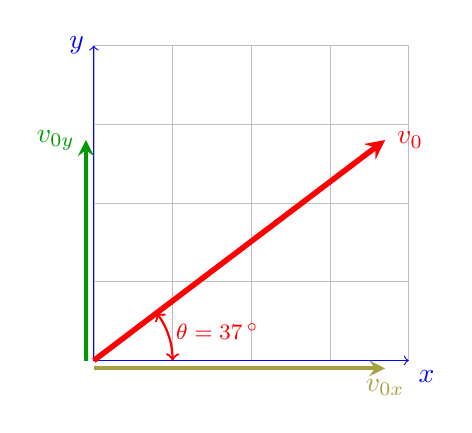
\begin{tikzpicture}[scale=1]
			\draw[very thin,color=gray!50] (0,0) grid (4,4);
			\draw[->, blue] (0,0) -- (4,0) node[below right] {$x$};
			\draw[->, blue] (0,0) -- (0,4) node[left] {$y$};
			\draw[-stealth,red, line width =2pt] (0,0) -- (3.7,2.8) node[right]{$v_0$};
			\draw[-stealth, line width = 1.5pt, green!60!black] (-.1,0) -- (-.1,2.8) node[left]{$v_{0y}$};
			\draw[-stealth, line width = 1.5pt, yellow!60!black] (0,-.1) -- (3.7,-.1) node[below]{$v_{0x}$};
			\draw[<->, red, thick] (1,0) arc (0:37.12:1cm) node[below right]{\ \footnotesize $\theta=37\,^\circ$};
		\end{tikzpicture}
	\end{center}
	
	Motion is split into $x$-component and $y$-component.  Typically, $x$ is horizontal (no acceleration) and $y$ is vertical (acceleration due to gravity, $a=-9.81\,\text{m/s}^2$).  If $v_0=12\,\text{m/s}$ and $\theta=37^\circ$,  the motion is:
	

		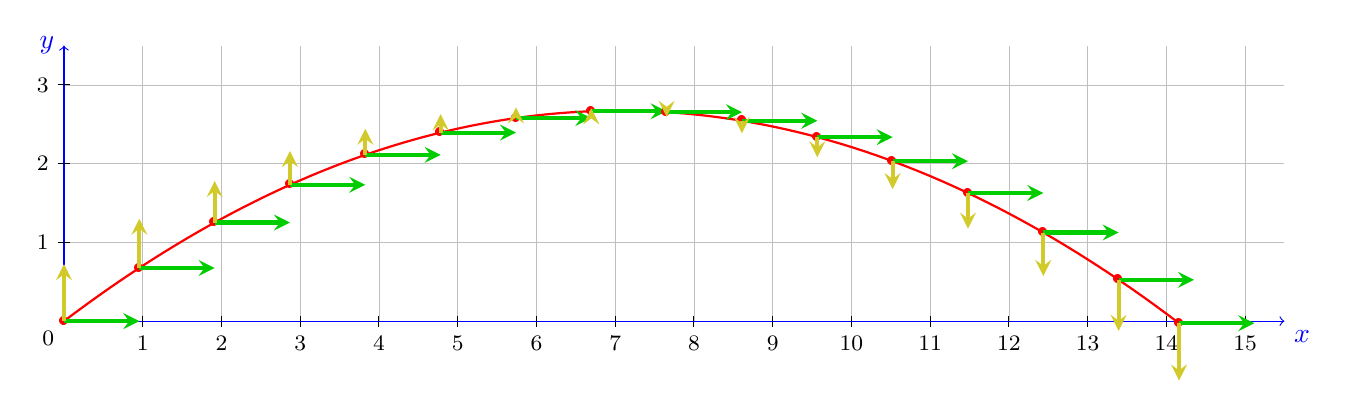
\begin{tikzpicture}[scale=1]
			\draw[very thin,color=gray!50,step=1cm] (0,0) grid (15.5,3.5);
			\draw[->, blue] (0,0) -- (15.5,0) node[below right] {$x$};
			\draw[->, blue] (0,0) -- (0,3.5) node[left] {$y$};
			\node[below left] at (0,0) {\footnotesize $0$};
			\foreach \x in {1,2,...,15}
			\draw[shift={(\x,0)}] (0pt,2pt) -- (0pt,-2pt) node[below] {\footnotesize $\x$};
			\foreach \x in {1,2,3}
			\draw[shift={(0,\x)}] (2pt, 0pt) -- (-2pt,0pt) node[left] {\footnotesize $\x$};
			\draw[red, thick, domain=0:1.48, samples=100] plot ({12*cos(37.12)*\x}, {-0.5*9.81*\x^2+12*sin(37.12)*\x});
			
			
			\foreach \x in {0,.1,.2,...,1.4,1.48}
			{
				\node at ({12*cos(37.12)*\x}, {-0.5*9.81*\x^2+12*sin(37.12)*\x})  {\footnotesize \textcolor{red}{\textbullet}};
				
				\draw[-stealth,green!80!black,line width=1.5pt] ({12*cos(37.12)*\x}, {-0.5*9.81*\x^2+12*sin(37.12)*\x}) -- ({12*cos(37.12)*\x+1.2*cos(37.12)}, {-0.5*9.81*\x^2+12*sin(37.12)*\x});
				
				\draw[-stealth,yellow!80!black,line width=1.5pt] ({12*cos(37.12)*\x}, {-0.5*9.81*\x^2+12*sin(37.12)*\x}) -- ({12*cos(37.12)*\x}, {(-0.5*9.81*\x^2+12*sin(37.12)*\x)+0.1*(-9.81*\x+12*sin(37.12))});	
			}
		\end{tikzpicture}
		where the arrows represent the \colorbox{pink!50}{\emph{velocity}} in the $x$- and $y$-directions.  The parametric equations for \colorbox{pink!50}{\emph{position} vs. time} are: $$\vec{x}=(12\cos\theta_0) t$$ and $$\vec{y}=(12\sin\theta_0) t-\frac{1}{2}\cdot9.81 t^2$$ where $\theta_0=37^\circ$
	\vspace{3cm}
	
	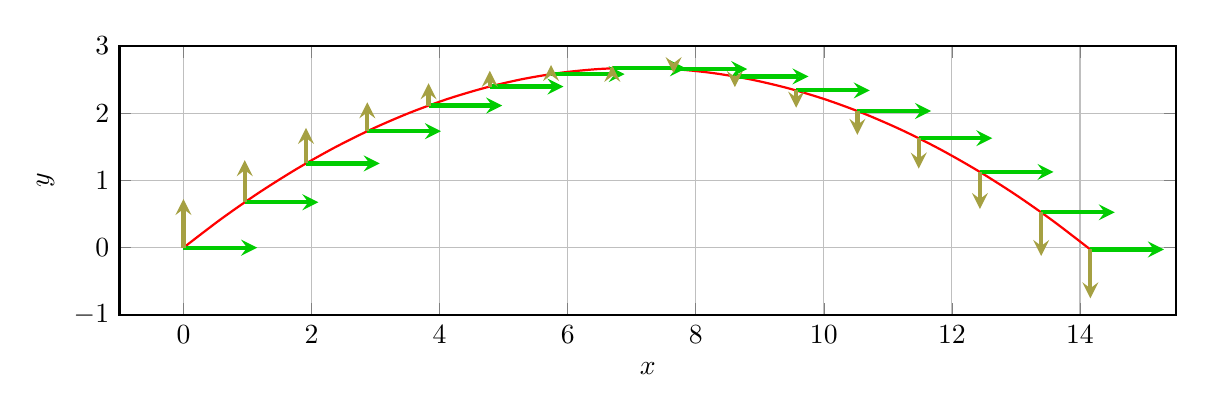
\begin{tikzpicture}
		\begin{axis}[width=15cm, height=5cm,xlabel={$x$}, ylabel={$y$},grid, thick,ymin=-1,
			ymax=3,
			xmin=-1,
			xmax=15.5]
			
			\addplot+[no marks,red,smooth,variable=t,domain=0:1.48]plot ({12*cos(37.12)*t}, {-0.5*9.81*t^2+12*sin(37.12)*t});
			
			\foreach \yValue in {0,.1,.2,...,1.4,1.48} {
				\edef\temp{\noexpand\draw [-stealth,green!80!black,line width=1.5pt] (axis cs:9.568*\yValue,-0.5*9.81*\yValue^2+12*0.6035*\yValue) -- (axis cs:1.2*.9586+9.568*\yValue,-0.5*9.81*\yValue^2+12*0.6035*\yValue);}
				\temp
				
				\edef\temp{\noexpand\draw[-stealth,yellow!60!black,line width=1.5pt] (12*.7974*\yValue, -0.5*9.81*\yValue^2+12*.6035*\yValue) -- (12*.7974*\yValue, -0.5*9.81*\yValue^2+12*.6035*\yValue+0.1*(-9.81*\yValue+12*.6035);}
				\temp
			}
		\end{axis}
		
	\end{tikzpicture}
\end{document}

